\documentclass[a4paper, 11pt]{article}
\usepackage[serbian]{babel}
\usepackage{hyperref}
\usepackage{graphicx}

\title{\large Seminarski rad iz predmeta Istra\v zivanje podataka 1
		\\ Podaci: FIFA19 }
\author{Nikola Jankovi\'c 
		\\ e-mail: \href{mailto:nikola_jankovic@tuta.io}{nikola\_jankovic@tuta.io}
		\\ \\ \small{Matemati\v cki fakultet, Univerzitet u Beogradu}
} 




\begin{document}


\begin{titlepage}
\maketitle
\thispagestyle{empty}

\begin{abstract}
Tema ovog seminarskog rada je detaljnija analiza, sa klasterovanjem,
skupa podataka dobijenog iz poslednje verzije
igrice FIFA19 (u toku pisanja rada) preuzetog sa adrese: \url{https://www.kaggle.com/karangadiya/fifa19}.
U radu \'{c}e biti prikazani neki od algoritama za klasterovanje i rezultati dobijeni primenom na ovaj skup.
Uz poku\v{s}aj da budu dobijeni klasteri što pribli\v{z}niji nekim podelama koje postoje u fudbalu. 
\end{abstract}

\end{titlepage}

\section{Uvod}



Klaster analiza je grupisanje objekata koje se oslanja samo na informacije koje se nalaze u podacima
koji opisuju te objekte i veze me\dj u njima. Cilj klaster analize je da objekti u grupi budu sli\v{c}ni(povezani) me\dj{}usobno i druga\v{c}iji od objekata u drugim grupama.
\v{S}to je ve\'{c}a sli\v{c}nost u grupi i razli\v{c}itost me\dj{}u grupama klaster analiza je 
izrazitija. \\
U ovom seminarskom radu bi\'{c}e prikazani rezultati klaster analize pomo\'{c}u algoritama
koji su vi\dj{}eni na kursu Istra\v{z}ivanje podataka 1:
\begin{itemize}
\item K-means
\item DBSCAN
\item Self Organizing Maps (\emph{Kohonen})
\item Hijerahijsko klasterovanje
\end{itemize} 
kao i dva dodatna algoritma:
\begin{itemize}
\item Mean-Shift
\item BIRCH
\end{itemize}


Svi algoritmi su primenjeni uz pomo\'{c} biblioteka jezika Python uz
kori\v{s}enje softvera IBM Spss Modeler zbog lo\v{s}e dokumentacije
vezane za SOM\footnote{Self Organizing Maps} u modulu \emph{minisom\footnote{\url{https://github.com/JustGlowing/minisom}}}.


\subsection{Skup podataka kori\v{s}\'{c}en u radu}
Skup podataka sastoji se od $\approx 18000$ igra\v{c}a(\emph{slogova}) i 89 ocena(\emph{atributa}).
Blagi uvid u tabelu je mogu\'{c} na slici 1. 
\begin{figure}[h]
\graphicspath{{../}}
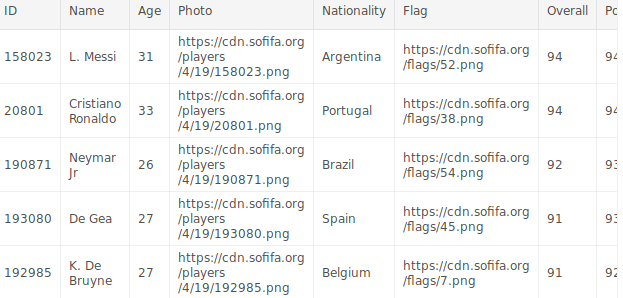
\includegraphics[scale=0.45]{head.png}
\caption{data.csv}
\label{data}
\end{figure}

Podaci iz skupa se koriste kao parametri koje koristi kompanija \emph{EA Sports}
pri kreiranju simulacije fudbalera iz realnog sveta kako bi napravili
distinkciju me\dj{}u njima.
\\
Nazivi kolona uglavnom nedvosmisleno ukazuju na njihovo zna\v{c}enje, ali \'{c}e 
ipak biti data obja\v{s}njenja za neke od atributa, koje korisnik smatra da nisu
poznati ve\'{c}ini.
\begin{itemize}

\item \emph{Value} - Predstavlja procenjenu trenutnu vrednost igra\v{c}a u dolarima, potrebno je praviti
razliku u odnosu na atribut \emph{Release Clause}

\item \emph{International Reputation} - Broj izme\dj{}u 0 i 1 koji govori koliko je uspeha imao u igrama za 
reprezentaciju svoje zemlje.

\item \emph{Loaned from} - Pojedini igra\v{c}i mogu biti posu\dj{}eni timu X od strane tima Y. Do kraja
posudbe tim X je u obavezi da pla\'{c}a igra\v{c}a u istom iznosu kao \v{s}to je to radio
tim Y. Na kraju posudbe tim X ima prednost (u nekim slu\v{c}ajevima i pravo) da otkupi u potpunosti
prava na igra\v{c}a od tima Y.

\item \emph{LS, ST, RS, ..., RB} - Atributi koji predstavljaju koliko je projektovana Overall ocena
igra\v{c}a u slu\v{c}aju da ga osoba koja igra igricu postavi na poziciju sa tim nazivom kolone.

\item \emph{Release Clause} - Procenjena cena koju je potrebno da tim Y plati timu X kako bi otkupio prava
na igra\v{c}a, \v{c}esto je vrednost ovog atributa ve\'{c}a u odnosu na atribut \emph{Value}, pogotovo kod
mla\dj{}ih igra\v{c}a.
\end{itemize}


\section{Analiza podataka}

U ovom delu bi\'{c}e izlo\v{z}ene neke zanimljive statistike iz skupa
i prikazano kako je izvr\v{s}eno pretprocesiranje podataka

\subsection{Statistike}
Na slici 2. mo\v{z}emo videti dijagaram zajedni\v{c}ke gustine raspodele
za ocene \emph{Overall} i \emph{Age}

\begin{figure}[h]
\centering
\graphicspath{{../}}
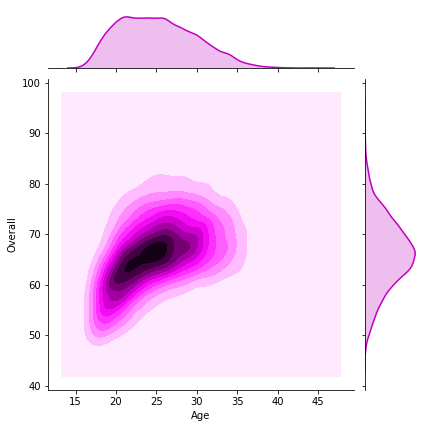
\includegraphics[scale=0.45]{stat1.png}
\caption{Dijagram odnosa Age $\sim$ Overall}

\end{figure}

Vidimo da je raspodela za \emph{Overall} normalna, dok
\emph{Age} podse\'{c}a na neku $\tilde{\chi}^2$ raspodelu.
Kao i da najve\'{c}i broj fudablera ima izme\dj{}u 23 i 27 godina
sa \emph{Overall} od 60 do 70 (potpuno o\v{c}ekivano).

\pagebreak

Druga zanimljiva statistika nam pokazuje raspodelu za atribut
\emph{Release Clause} i lako se uo\v{c}ava da najve\'{c}a koli\v{c}ina
novca figurira  u malom procentu igra\v{c}a. Dok je kod igra\v{c}a
koji nisu vrhunske klase to zna\v{c}ajno manje.


\begin{figure}[h]

\graphicspath{{../}}
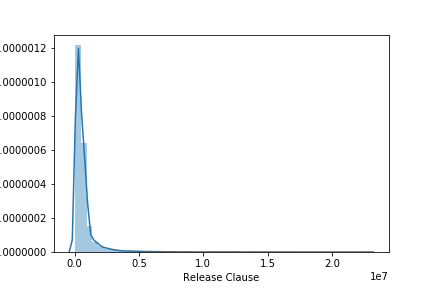
\includegraphics[scale=0.45]{stat2.png}
\caption{Raspodela izlazne klauze}

\end{figure}




I tre\'{c}i dijagram nam pokazuje koliko igra\v{c}a nam dolazi 
iz koje dr\v{z}ave (razmatrane samo dr\v{z}ave koje imaju vi\v{s}e od 500 predstavnika)


\begin{figure}[h]
\centering
\graphicspath{{../}}
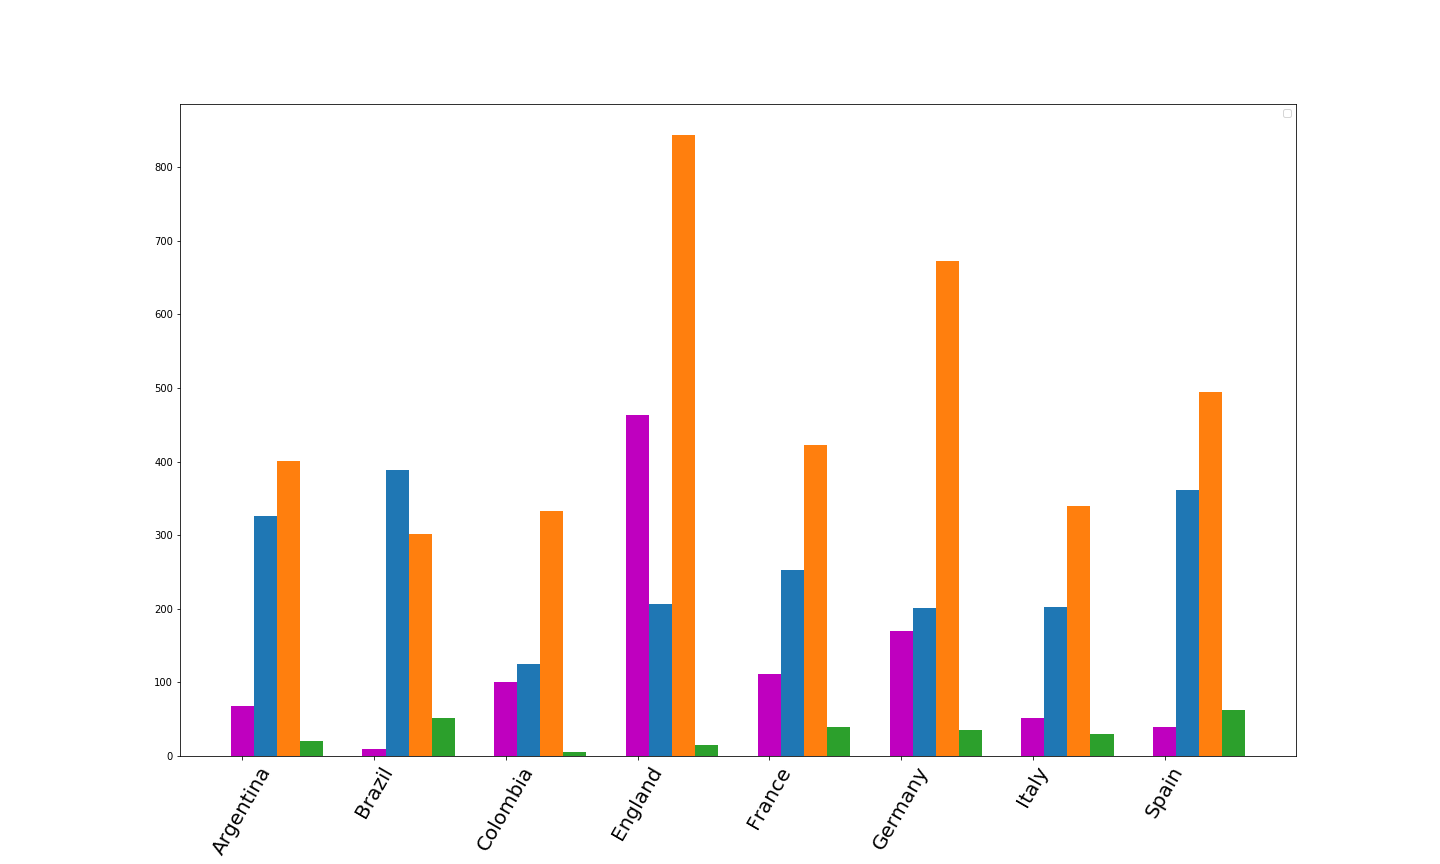
\includegraphics[scale=0.285]{stat3.png}
\caption{}

\end{figure}

Primetno je da je broj igra\v{c}a iz Engleske najve\'{c}i kao
i da dominiraju u broju igra\v{c}a sa ocenom manjom od 60.
Razlog ovome je to \v{s}to u igrici postoje timovi iz \v{c}ak
4 engleska liga\v{s}ka takmi\v{c}enja u kojima ve\'{c}inu \v{c}ine
igra\v{c}i iz Engleske, a kako su timovi iz 3. i 4. ranga polu-profesionalni,
ocene za igra\v{c}e su o\v{c}ekivano niske.
\pagebreak

\subsection{Pretprocesiranje}

\end{document}